\mychapter{Metodologia}

%pode apagar!
Para alterar este texto basta dar um 
\textbf{duplo clique “aqui”}, e o local de edição será aberto na sua caixa de edição do lado “esquerdo”.

%pode apagar tudo!
\textbf{Copie e cole seu texto aqui.}

\textbf{Para mudar a imagem basta alterar o caminho contido no comando "linewidth ${figuras/abntex2-modelo-img-grafico.pdf}$" para a imagem desejada.}

\textbf{OBS: todas as imagens devem ser colocadas na pasta figures, para isso basta clicar na pasta e clicar no botão Upload localizado no menu superior a esquerda. 
}

\begin{figure}[H]
\begin{center}
\caption{EXEMPLO DE FIGURA - TODO ESCRITO EM CAIXA ALTA.}
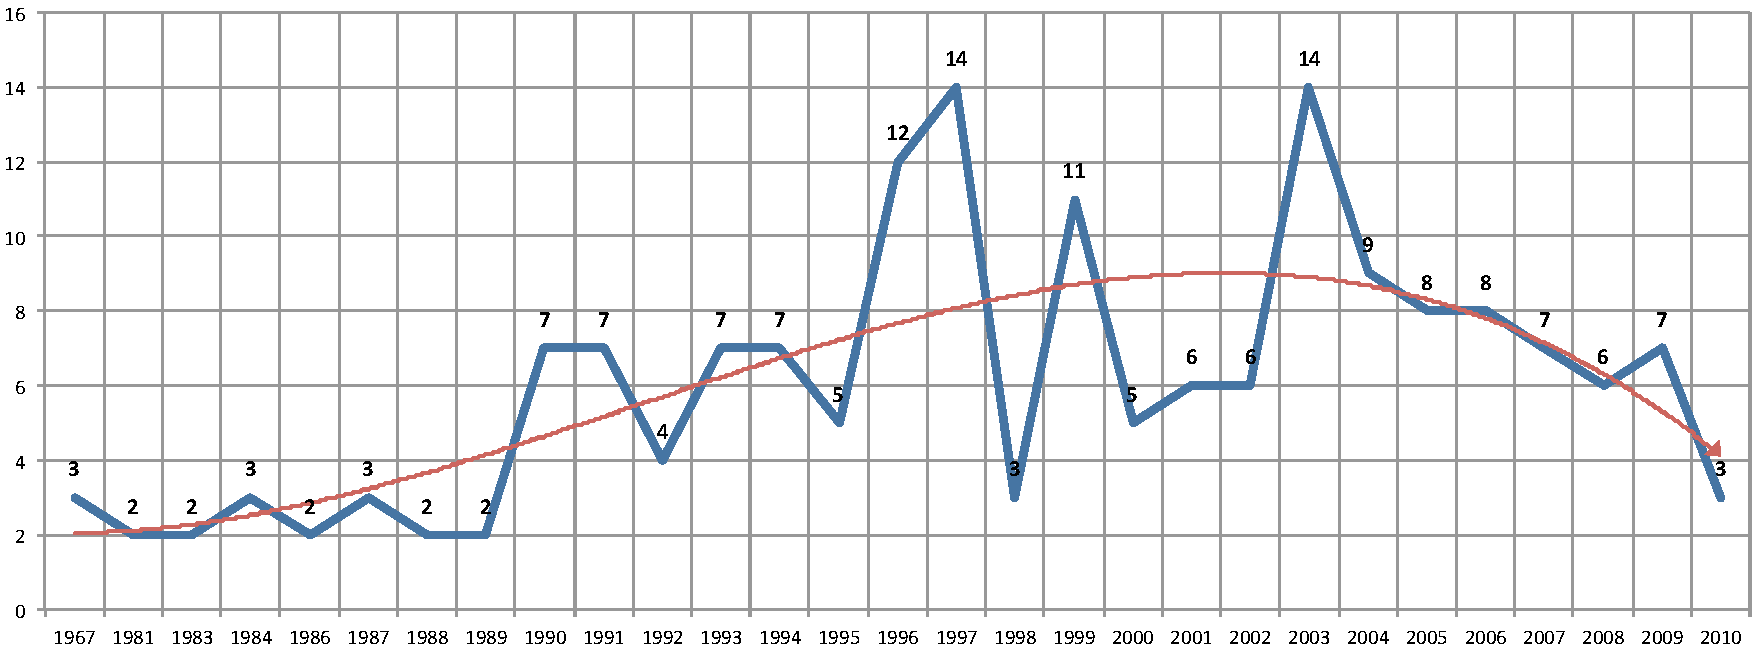
\includegraphics[width=12cm]{figuras/abntex2-modelo-img-grafico.pdf}
\legend{Fonte: Adaptado de \citeonline{NBR14724:2011}.}
\label{fig:controleUComparativo}
\end{center}
\end{figure}

